\documentclass[11pt]{article}
\usepackage[spanish, es-tabla, es-lcroman]{babel}

%Paquetes básicos
\usepackage{multicol}
\usepackage{physics} 
\usepackage{float}
\usepackage{gensymb}
\usepackage{siunitx} 
\usepackage{enumerate} 
\usepackage{url}
\usepackage{pgfplots}
\usepackage{pgfplotstable}
\usepackage{tikz,pgfplots}
\usepackage{amsmath}  
\usepackage{wasysym} 
\usepackage{geometry}
\usepackage{mdframed}
%Fuente: Helvetica
\usepackage[scaled]{helvet}
\usepackage[T1]{fontenc}
\renewcommand\familydefault{\sfdefault}
\usepackage[eulergreek]{sansmath}
\usepackage[frenchmath]{newtxsf}
\renewcommand{\familydefault}{\sfdefault}
\usepackage{mathastext}
\usepackage{lipsum}
\usepackage{apacite}
\usepackage{natbib}

%Paquetes necesarios para la elaboración de Figuras con el ambiente tikzpicture
\usepackage{tikz} 
\tikzset{font=\fontfamily{phv}\selectfont}
\usepackage{amsmath,tikz}
\usepackage{tikz-3dplot}
\usetikzlibrary{calc,positioning,intersections}
\usetikzlibrary{positioning,shapes.misc}
\tdplotsetmaincoords{80}{120}
\usetikzlibrary{decorations.markings} 
\usetikzlibrary{decorations.pathmorphing}
\usetikzlibrary{shapes, shapes.geometric}
\usetikzlibrary{mindmap,trees}
\usetikzlibrary{backgrounds, fit, positioning}
\tikzstyle{flecha} = [thick,->,>=stealth]


%Geometría de la página y encabezados
\geometry{a4paper,top=3cm,bottom=2.5cm,right=2.5cm,left=2.5cm}
\pgfplotsset{compat=1.14}
\pgfplotsset{/pgf/number format/use comma}
%Estilo de encabezados
\usepackage{fancyhdr}
\pagestyle{fancy}
\fancyhf{}
\lhead{IA Fundamentals}
\rhead{Maestría en CD-IA / UTEC}
\cfoot{\thepage}




%-----------------------
%AQUÍ SE DEBE REEMPLAZAR EL SÍMBOLO NUMERAL POR EL NÚMERO DE LA PRÁCTICA
\chead{Práctica N$^{\circ}$\01}
%-----------------------



%Configuración del estilo de los títulos de las secciones y subsecciones
\usepackage{titlesec}
\titleformat{\section}{\normalfont\normalsize\bfseries\centering}{\thesection.}{0.5em}{}
\titleformat{\subsection}{\normalfont\normalsize\bfseries}{\thesubsection.}{0.5em}{}



%-----------------------
%AQUÍ SE DEBE REEMPLAZAR LO ESCRITO POR EL TÍTULO DE LA PRÁCTICA
\title{\LARGE\textbf{Sistema Experto: Recomendación de Medicamentos}}
%-----------------------



%-----------------------
%Y LOS NOMBRES DE CADA UNO DE LOS INTEGRANTES DEL GRUPO
\author{\normalsize{Silupu Peñaranda, Collin Rodrigo $\cdot$ 202431053}}
%-----------------------


\date{\small{\today}}

\begin{document}
\renewcommand{\BOthers}[1]{et al.\hbox{}}


\maketitle


\hrule

\begin{abstract}
\noindent %En general, el resumen no contiene sangría, el comando noident se encarga de no poner la sangría al párrafo
El sistema experto propuesto utiliza un conjunto de reglas para determinar qué medicamento recomendar en función de las respuestas a una serie de preguntas sobre síntomas y enfermedades.
Es importante destacar que el sistema no se centra en determinar si el medicamento recomendado es el más indicado para una condición específica. La finalidad del sistema es demostrar que puede generar recomendaciones basadas en una base de datos de información preestablecida, y probar su funcionalidad, mas no para ofrecer consejos médicos verificados. Por ello, se recomienda encarecidamente que cualquier implementación real de este sistema en entornos clínicos sea acompañada por la supervisión y validación de especialistas en el área médica.

\noindent\textit{\textbf{Palabras claves:} sistema experto, medicamentos, recomendación.}

\end{abstract}

\hrule

\begin{multicols}{2}
\section{Introducción}
En el ámbito de la salud, la precisión y eficacia en la administración de tratamientos médicos es crucial. Frente a un amplio espectro de enfermedades y condiciones médicas, los profesionales de la salud a menudo se enfrentan al desafío de seleccionar el medicamento más adecuado basándose en los síntomas y antecedentes del paciente. Este proceso, si bien es fundamental, puede ser propenso a errores y consumir un tiempo valioso. Además, con el crecimiento de la telemedicina y la consulta en línea, la necesidad de sistemas automatizados y confiables para la recomendación de tratamientos se ha vuelto más apremiante.

En este contexto, se desarrolló un sistema experto experimental destinado a automatizar la recomendación de medicamentos basándose en los síntomas reportados por el usuario y otras variables de diagnóstico relevantes. La finalidad de este sistema es proporcionar una herramienta de apoyo para los profesionales de la salud que mejore la eficiencia y precisión en la prescripción de tratamientos, al mismo tiempo que minimiza los riesgos asociados con la selección incorrecta de medicamentos\footnote{El propósito de este sistema es demostrar su capacidad para generar recomendaciones basadas en una base de datos de información preestablecida y probar su funcionalidad, sin proporcionar consejos médicos especializados.}.

Un sistema experto es un sistema informático diseñado para replicar las habilidades de toma de decisiones de expertos humanos. Utiliza conocimientos especializados y procedimientos de inferencia para abordar problemas complejos que normalmente requieren experiencia humana. Los sistemas expertos operan dentro del ámbito de la inteligencia artificial (IA) y tienen como objetivo funcionar como seres humanos expertos en escenarios de resolución de problemas \citep{suryadi, lestari}. 

Estos sistemas se basan en un repositorio de conocimiento experto, que puede incluir datos de libros, revistas y la experiencia de especialistas humanos. Al aprovechar este conocimiento especializado, los sistemas expertos permiten a las personas resolver problemas a nivel de expertos o acceder a información de alta calidad que de otro modo requeriría asistencia experta \citep{suryadi, lestari}.

En este sentido, el presente sistema se basa en un conjunto de reglas definidas que evalúan las respuestas del usuario a una serie de preguntas relacionadas a su estado de salud actual. Estas preguntas abarcan desde síntomas generales, hasta condiciones médicas específicas. El motor de inferencia del sistema utiliza estas respuestas para activar reglas específicas que concluyen con la recomendación de un medicamento o un conjunto de medicamentos que correspondan a las necesidades del usuario.


\section{Descripción del Sistema Experto}

El sistema experto está diseñado para ofrecer recomendaciones de medicamentos basándose en un conjunto de reglas que evalúan las respuestas del usuario a una serie de preguntas sobre los malestares que presenta. En este sentido, este sistema sigue el enfoque forward chaining (encadenamiento hacia adelante), dado que comienza con un conjunto de hechos o datos y aplica reglas para inferir conclusiones a partir de esos datos. Cabe resaltar que el arbol de decisión se encuentra en la imagen del Anexo \ref{fig:miImagen}


\subsection{Estructura del Árbol de Decisión}
El sistema utiliza un árbol de decisión que inicia con una pregunta fundamental: "¿Te sientes enfermo en este momento?". Según la respuesta del usuario, el sistema se bifurca hacia dos diferentes caminos:
\begin{itemize}
    \item Si el usuario indica que no se siente enfermo, el sistema concluye con un ``¡Gracias a Dios!'' como respuesta final.
    \item Si el usuario confirma que se siente enfermo, el sistema procede a realizar preguntas más detalladas para identificar síntomas específicos como fiebre, dolor o inflamación.
\end{itemize}

\subsection{Identificación de Síntomas}
Dependiendo de las respuestas a las preguntas iniciales, el sistema pregunta sobre síntomas adicionales y condiciones específicas, como infecciones bacterianas. Cada respuesta lleva a una recomendación de medicamento específico. 
\begin{itemize}
    \item Ibuprofeno se recomienda si hay dolor, fiebre e inflamación.
    \item Paracetamol se sugiere para el dolor y la fiebre sin inflamación.
    \item Aspirina para el dolor y la inflamación sin fiebre.
    \item Amoxicilina se prescribe en caso de diagnóstico de infección bacteriana sin dolor.
\end{itemize}

\subsection{Identificación de Condiciones Médicas}
Sin importar si es que el sistema identifique si el usuario, en el momento de la ejecución, está enfermo o no, realiza una serie de preguntas para identificar condiciones médicas específicas. En este sentido, se busca recomendar un medicamento específico a cada condición médica.
\begin{itemize}
    \item Loratadina se utiliza para el tratamiento de alergias, incluyendo síntomas como estornudos y picazón.
    \item Metformina es recomendada para pacientes con diabetes tipo 2, ayudando a mejorar el control del azúcar en sangre.
    \item Omeprazol se aconseja para el tratamiento de la acidez estomacal y las úlceras gástricas.
    \item Simvastatina se utiliza para reducir los niveles de colesterol alto y prevenir enfermedades cardiovasculares.
    \item Ciprofloxacino se recomienda para tratar infecciones bacterianas.
    \item Diclofenaco se sugiere para aliviar el dolor, la inflamación y los síntomas de artritis.
    \item Alprazolam se prescribe para el manejo de la ansiedad y trastornos de pánico.
    \item Sertralina se utiliza en el tratamiento de la depresión, trastorno obsesivo-compulsivo y la ansiedad.
    \item Amlodipina se emplea en el tratamiento de la presión arterial alta.
    \item Montelukast se recomienda para el manejo del asma y otras alergias.
    \item Prednisona se utiliza para tratar inflamaciones severas y condiciones autoinmunes.
    \item Fluconazol se administra para combatir infecciones fúngicas.
    \item Ranitidina se utiliza para tratar úlceras y la enfermedad de reflujo gastroesofágico.
    \item Losartán se prescribe para controlar la presión arterial alta.
    \item Clotrimazol se recomienda para tratar infecciones fúngicas en la piel, boca y genitales.
    \item Venlafaxina se utiliza para el tratamiento de la depresión mayor y trastorno de ansiedad generalizada.
\end{itemize}

Es importante destacar que la información sobre los usos y efectos de los medicamentos presentada en este documento ha sido obtenida a través de ChatGPT \citep{chatgpt}. Por lo tanto, no debe considerarse como una fuente médica confiable y verificada. La intención de incluir estos ejemplos es meramente ilustrativa, con el objetivo de demostrar la potencial utilidad de un sistema experto en el ámbito de la salud. Este sistema debería ser implementado utilizando información fiable y verificada por profesionales médicos para garantizar su precisión y seguridad. La efectividad de un sistema experto depende en gran medida de la calidad y veracidad de los datos que se utilizan para alimentarlo. Por ello, se recomienda encarecidamente que cualquier implementación real de este sistema en entornos clínicos sea acompañada por la supervisión y validación de especialistas en el área médica.

\section{Resultados}
En esta sección se presentarán los resultados obtenidos de la ejecución práctica del sistema experto desarrollado para la recomendación de medicamentos basado en síntomas específicos. Este análisis se ilustra a través de capturas de pantalla que documentan las interacciones típicas entre el usuario y el sistema, destacando cómo este último procesa las entradas y llega a conclusiones lógicas sobre el tratamiento adecuado.

En la imagen del Anexo \ref{fig:imagen1}, se observa que si el usuario marca No cuando se le presenta la pregunta si está enfermo en el momento de la ejecución el sistema arroja un "Gracias a Dios". Asimismo, el sistema le plantea la primera pregunta sobre si sufre o no alguna de esas condiciones médicas, tal y como se planteó en la sección anterior. 

En la imagen del Anexo \ref{fig:imagen2}, se observan las cinco preguntas que se plantean sobre las condiciones médicas. Si el usuario decide responder "Ninguna de las anteriores en todas", el sistema arroja el mensaje de "Gracias a Dios". Cabe resaltar que en cada pregunta, si el usuario responde "Ninguna de las anteriores", el sistema arrojará el mensaje "Responda la siguiente pregunta". 

En la imagen del Anexo \ref{fig:imagen3}, se observa que al presentársele la pregunta inicial sobre si se siente enfermo, y el usuario responde afirmativamente (indicado como Sí), el sistema procede a interrogar sobre la presencia de dolor. La respuesta del usuario a esta pregunta se puede marcar con un Sí o con un No. En caso de que la respuesta sea Sí, se formula una pregunta subsiguiente sobre la presencia de fiebre. Si la respuesta es No, entonces se plantea una consulta adicional acerca de si el usuario está experimentando inflamación. Si el usuario responde Sí a esta última, el sistema concluye que el tratamiento adecuado sería la administración de Aspirina, como se mencionó en la sección anterior, recomendada específicamente para casos de dolor e inflamación en ausencia de fiebre. Asimismo, se plantea de igual manera la primera pregunta sobre condiciones médicas.

En la imagen del Anexo \ref{fig:imagen4}, se observa que si el usuario sigue con la interacción, y responde que, por ejemplo, presenta Diabetes Tipo 2, automáticamente el sistema recomendará la toma de Metformina, asimismo, se abrirá la siguiente sección de preguntas. Si en esta última, el usuario señala que presenta dolores, inflamación y artritis, el sistema recomendará la toma de Diclofenaco. Además, se abre la siguiente sección de preguntas, y si el usuario señala que si el usuario sufre de depresión y de desórdenes obsesivos compulsivos, el sistema recomendará la toma de Sertralina. El resto de preguntas se irán abriendo a medida que el usuario vaya respondiendo. 

Si el usuario ahora señala no sentirse mal en el momento de la ejecucion; sin embargo, es paciente de algun diagnóstico en específico, como por ejemplo Asma o Alergias, el sistema automáticamente le recomendará tomar Montelukast, el cual es recomendable en casos de asma y alergias (Ver imagen del Anexo \ref{fig:imagen5}).

En este sentido, los resultados planteados en esta sección muestran la capacidad del sistema para procesar información y llegar a conclusiones lógicas sobre tratamientos adecuados, demostrando utilidad clínica potencial. Cabe resaltar que la precisión de las recomendaciones depende de la exhaustividad de la base de datos, siendo una limitación a considerar

\section{Conclusiones}

El sistema experto está diseñado para ofrecer recomendaciones de medicamentos y se basó en un conjunto de reglas que evalúan las respuestas del usuario a una serie de preguntas sobre los malestares que presenta. Los resultados obtenidos validan la eficacia del enfoque de encadenamiento hacia adelante empleado por el sistema, permitiendo la activación secuencial de reglas en respuesta a la información ingresada por el usuario. 

Las pruebas realizadas en la sección de resultados, muestra la capacidad del sistema experto para recomendar medicamentos basados en los síntomas y condiciones médicas proporcionados por el usuario. Estas interacciones ilustran cómo el sistema procesa las entradas del usuario y llega a conclusiones lógicas sobre el tratamiento adecuado. A través de diferentes escenarios, como la presencia de síntomas específicos o diagnósticos médicos preexistentes, el sistema ofrece recomendaciones de medicamentos correspondientes. Estos resultados sugieren que el sistema puede realizar recomendaciones similares para una amplia gama de diagnósticos y malestares planteados en la base de datos, demostrando su utilidad potencial en la práctica clínica. Sin embargo, 

En cuanto a las limitaciones, es importante tener en cuenta que la efectividad del sistema depende en gran medida de la precisión y exhaustividad de la base de datos proporcionada, lo que puede limitar su capacidad para abordar ciertos diagnósticos o malestares menos comunes o no incluidos en la base de datos. Por otro lado, es crucial subrayar que la implementación de este sistema en un entorno clínico requiere una base de datos médica verificada y actualizada, ya que la confiabilidad de las recomendaciones depende intrínsecamente de la calidad de la información médica utilizada. En cuanto al presente sistema experto, se utilizaron datos no verificados, los cuales fueron proporcionados por ChatGPT; por ello, es recomendable plantear la importancia de la colaboración con profesionales médicos para validar y enriquecer el contenido del sistema.





\bibliographystyle{apacite} 
\bibliography{referencias.bib}

\end{multicols}






\section{Anexo}

\subsection{Anexo 1}
\begin{figure}[H]
  \centering
  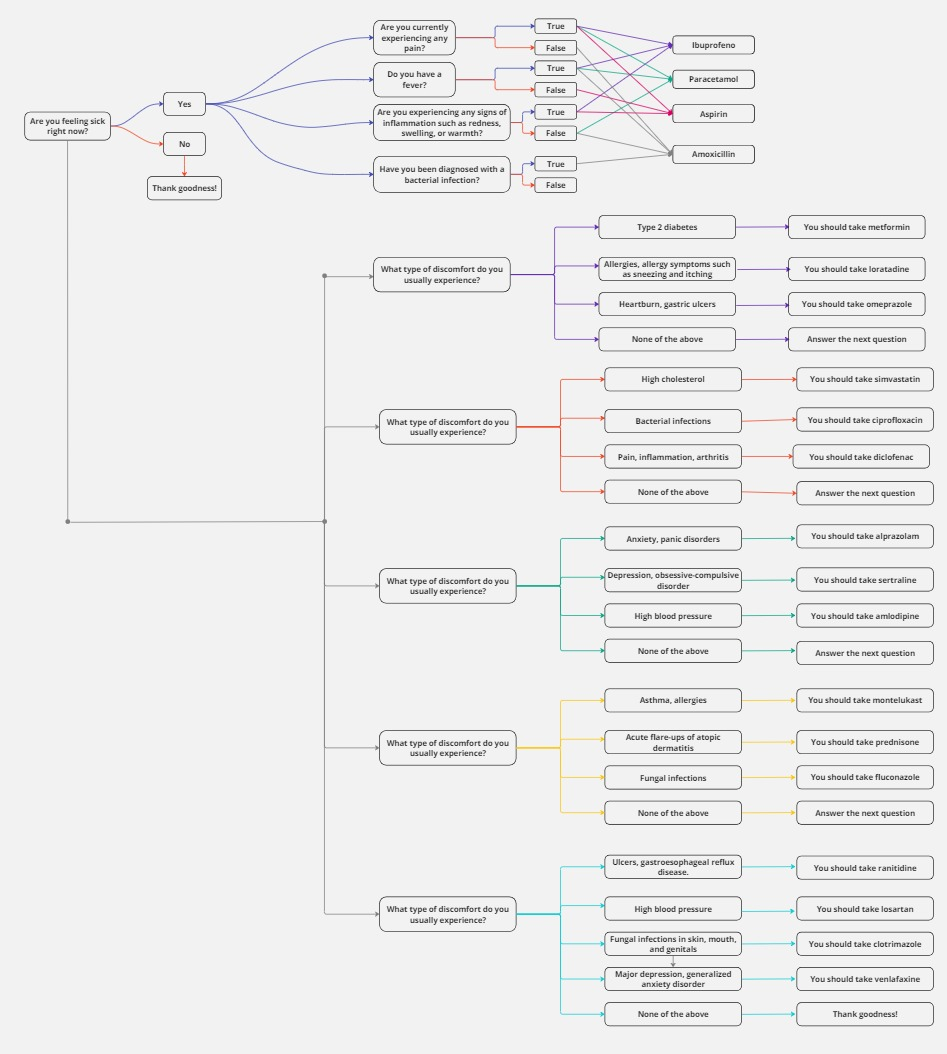
\includegraphics[width=\linewidth]{Graphs/SE_RM.jpg}
  \label{fig:miImagen}
\end{figure}

\subsection{Anexo 2}
\begin{figure}[H]
  \centering
  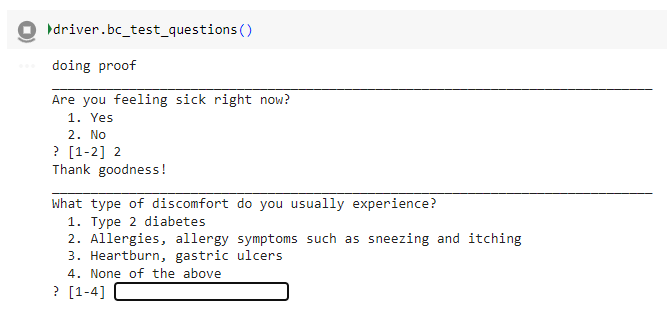
\includegraphics[width=\linewidth]{Graphs/imagen1.png}
  \label{fig:imagen1}
\end{figure}

\subsection{Anexo 3}
\begin{figure}[H]
  \centering
  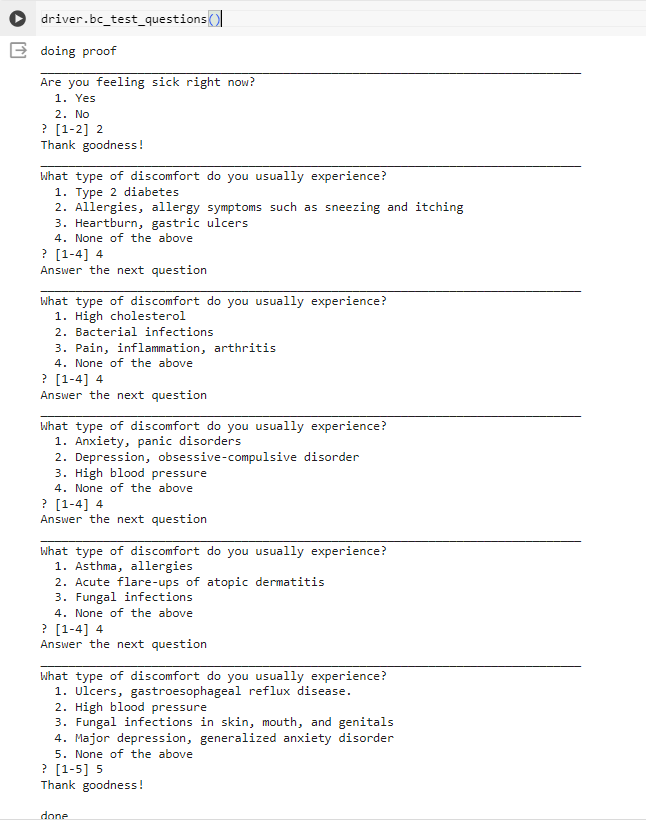
\includegraphics[width=\linewidth]{Graphs/imagen2.png}
  \label{fig:imagen2}
\end{figure}

\subsection{Anexo 4}
\begin{figure}[H]
  \centering
  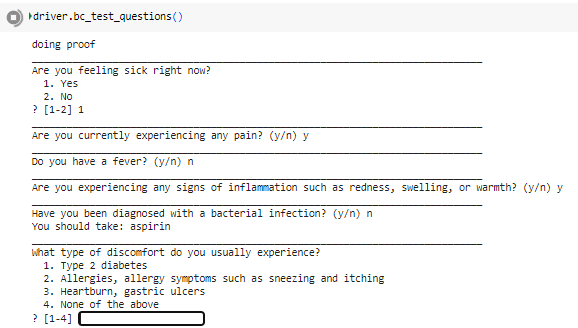
\includegraphics[width=\linewidth]{Graphs/imagen3.png}
  \label{fig:imagen3}
\end{figure}

\subsection{Anexo 5}
\begin{figure}[H]
  \centering
  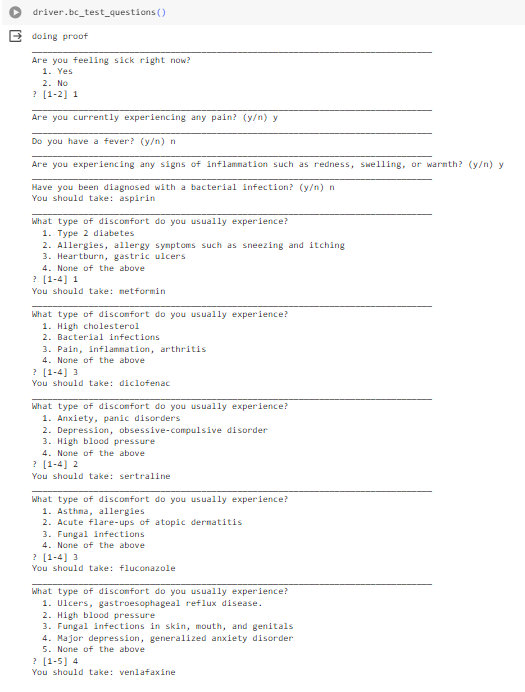
\includegraphics[width=\linewidth]{Graphs/imagen4.png}
  \label{fig:imagen4}
\end{figure}

\subsection{Anexo 6}
\begin{figure}[H]
  \centering
  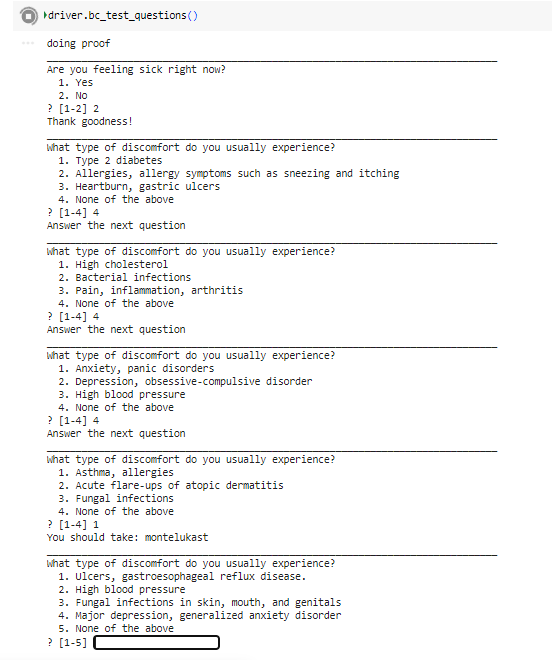
\includegraphics[width=\linewidth]{Graphs/imagen5.png}
  \label{fig:imagen5}
\end{figure}


\end{document}
